\documentclass[journal]{vgtc} 
\usepackage{hs-vis_ss10}


%% Please note that the use of figures other than the optional teaser
%% is not permitted on the first page of the journal version.  Figures
%% should begin on the second page and be in CMYK or Grey scale
%% format, otherwise, colour shifting may occur during the printing
%% process.  Papers submitted with figures other than the optional
%% teaser on the first page will be refused.

%% These three lines bring in essential packages: ``mathptmx'' for
%% Type 1 typefaces, ``graphicx'' for inclusion of EPS figures. and
%% ``times'' for proper handling of the times font family.

\usepackage{mathptmx} 
\usepackage{graphicx}
\usepackage{times}
\usepackage{amssymb}
\usepackage{amsmath}
\usepackage{mathtools}
\usepackage{bigints}
\usepackage{xfrac}
\usepackage{bm}
\usepackage{cleveref}
\usepackage{csquotes}
\usepackage{subcaption}
\usepackage[english]{babel}

\DeclareMathAlphabet{\mathcal}{OMS}{cmsy}{m}{n}

\newcommand{\lam}{\lambda}
\newcommand{\trans}{\quad\bigg|\;}
\newcommand{\Trans}{\quad\Bigg|\;}
% matrix shortcut
\newcommand{\mat}[1]{\begin{pmatrix} #1 \end{pmatrix}}
% matrix shortcut with increased vertical spacing
\newcommand{\Mat}[1]{\begingroup
\renewcommand*{\arraystretch}{1.5}
\mat{#1}
\endgroup}
% matrix format but without braces (secretly a matrix)
\newcommand{\secretMat}[2][r]{\begin{matrix*}[#1] #2 \end{matrix*}}
% matrix format but without braces (secretly a matrix) with increased vertical spacing
\newcommand{\SecretMat}[2][r]{\begingroup
\renewcommand*{\arraystretch}{1.7}
\secretMat[#1]{#2}
\endgroup}
% shortcuts for df/dx stuff in derivative
\newcommand{\der}{\partial}
\newcommand{\deriv}[2]{\frac{\der #1}{\der #2}}
% make star '*' become \cdot (normal multiplication sign)
\mathcode`\*="8000
{\catcode`\*\active\gdef*{\cdot}}
\newcommand{\Real}{\mathbb{R}}
\newcommand{\flow}{\vec{u}}
\newcommand{\x}{\vec{x}}
\newcommand{\y}{\vec{y}}
\newcommand{\ev}{\vec{r}}
\newcommand{\aaux}{\vec{a}}
\newcommand{\baux}{\vec{b}}
\newcommand{\T}{^\top}
\newcommand{\argmin}{\mathop{\mathrm{argmin}}}
\newcommand{\charbonnier}{\psi_{\text{Ch}}}
\newcommand{\peronamalik}{\psi_{\text{PM}}}
\newcommand{\Rfirst}{R_{1\text{st}}}
\newcommand{\Rsecond}{R_{2\text{nd}}}
\newcommand{\jacob}{\mathcal{J}}
\newcommand{\patch}{\mathcal{N}}
\newcommand{\cnl}{c_{\text{nl}}}
\newcommand{\cNl}{\overset{\_}{c}_{\text{nl}}}



%% allow for this line if you want the electronic option to work
%% properly
\vgtcinsertpkg


%% author name
\author{David H\"agele}

%% paper title
\title{An Elaboration on\\Order-Adaptive Regularisation for Variational Optical Flow:\\Global, Local and in Between}

%% short title for header
\shorttitle{Order-Adaptive Regularisation}


%% Abstract section.
\abstract{%
  Hier sollte eine kurze Zusammenfassung der Ausarbeitung stehen. Der
  Umfang sollte 150 bis 250 Worte betragen. Duis autem vel eum iriure
  dolor in hendrerit in vulputate velit esse molestie consequat, vel
  illum dolore eu feugiat nulla facilisis at vero eros et accumsan et
  iusto odio dignissim qui blandit praesent luptatum zzril delenit
  augue duis dolore te feugait nulla facilisi. Lorem ipsum dolor sit
  amet, consectetuer adipiscing elit, sed diam nonummy nibh euismod
  tincidunt ut laoreet dolore magna aliquam erat volutpat.

  Ut wisi enim ad minim veniam, quis nostrud exerci tation ullamcorper
  suscipit lobortis nisl ut aliquip ex ea commodo consequat. Duis
  autem vel eum iriure dolor in hendrerit in vulputate velit esse
  molestie consequat, vel illum dolore eu feugiat nulla facilisis at
  vero eros et accumsan et iusto odio dignissim qui blandit praesent
  luptatum zzril delenit augue duis dolore te feugait nulla facilisi.
} % end of abstract


%% Uncomment below to include a (optional) teaser figure.
%\teaser{ \centering
%  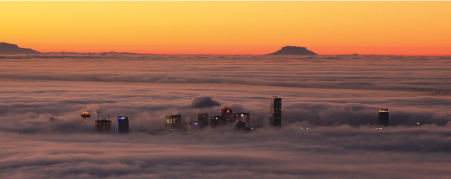
\includegraphics[width=16cm]{images/CypressView}
%  \caption{In den Wolken: Vancouver von Cypress Mountain. Auf der
%    ersten Seite d"urfen keine Grafiken au"ser dieser optionalen
%    Aufmachgrafik (Teaser) abgebildet sein.}
%}


%%%%%%%%%%%%%%%%%%%%%%%%%%%%%%%%%%%%%%%%%%%%%%%%%%%%%%%%%%%%%%%%
%%%%%%%%%%%%%%%%%%%%%% START OF THE PAPER %%%%%%%%%%%%%%%%%%%%%%
%%%%%%%%%%%%%%%%%%%%%%%%%%%%%%%%%%%%%%%%%%%%%%%%%%%%%%%%%%%%%%%%%

\begin{document}

%% The ``\maketitle'' command must be the first command after the
%% ``\begin{document}'' command. It prepares and prints the title
%%   block.

%%   the only exception to this rule is the \firstsection command
\firstsection{Introduction}

\maketitle

In computer vision, the field of optic flow deals with the estimation of a 2-dimensional flow field based on two consecutive frames of an image sequence.
\\(mehr dazu warum optic flow geil ist)\\
Different methods for flow estimation exist, such as ... ... and variational optic flow which is based on the calculus of variations.
In the following the concept of variational flow estimation is recapitulated and the approach by Maurer, Stoll and Bruhn \cite{daspaper} with order adaptive regulalarization is presented.

\section{Variational Optic Flow}\label{sec:variationalopticflow}
In this section the general framework for flow estimation using variational methods is recapitulated.
\\\\
Given two subsequent images of an image sequence\\
$I_0,I_1 ~:~ \Omega \subset \Real^2 \to \Real$,\\
we seek the displacement vector field 
\\$\flow = (u~v)\T ~:~ \Omega \subset \Real^2 \to \Real^2$\\
that maps $I_0$ onto $I_1$ such that
\\$I_0(\x) = I_1(\x+\flow(\x))$.
\\\\
To estimate the flow function $\flow$ an energy functional is minimized. 
Typically this functional consists of two terms, a data term $D(\flow)$ and a regularization term $R(\flow)$.
\begin{flalign*}
\flow' &= \argmin_{\flow} E(\flow)&&
\\
E(\flow) &= D(\flow) + \alpha R(\flow)&&
\end{flalign*}
In this framework, the data term is used to penalize flow functions which violate certain constancy assumptions on image features, such as the brightness constancy assumtion. 
\begin{flalign*}
D_{brght}(\flow) = \int_\Omega (I_0(\x)-I_1(\x+\flow(\x))^2\;d\x&&
\end{flalign*}
As the data term is insufficient for solving this problem and would yield multiple ambiguous solutions as illustrated in \cref{fig:ambigdataterm}, the regularization term is used to overcome this inconvenience and penalize flow functions that are unlikely.
This is done by setting up constraints for the flow, such as the first order smoothness assumption.
\begin{flalign*}
R_{smooth}(\flow) = \int_\Omega || \nabla u ||_2^2 + || \nabla v ||_2^2\;d\x&&
\end{flalign*}
This assumption enforces constant flow due to penalizing non vanishing gradients, which amount to changes in the vector field.
\begin{figure}[htb]
\centering
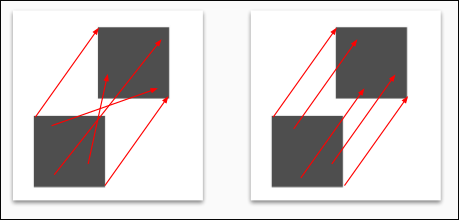
\includegraphics[width=\linewidth]{images/ambiguousflow.png}
\caption{Images show a rectangle that moved from bottom left to top right. The red arrows sketch a flow field explaining where the pixels moved.
Even though both fields perfectly fulfill a data term with brightness and gradient constancy assumption, only the right field is reasonable and would minimize a first order smoothness regularization.}
\label{fig:ambigdataterm}
\end{figure}

In order to minimize the energy functional, an iterative update sheme is developed using the Euler-Lagrange equation \cite{mathforphysicists}.

\section{Motivation}\label{sec:motivation}
As explained in \cref{sec:variationalopticflow} the regularization term can be used to constrain the \enquote{type} of the estimated flow function.
In practice either first or second order smoothness assumptions are made in which a flow function minimizes the regularization term when its first or second derivative vanishes.
Therefore, first order methods are suitable for motion that is constant, i.e. parallel to the image plane.
Second order methods can be leveraged for estimating affine flow fields as the class of linear functions implies vanishing second derivative.
\Cref{fig:flowfields} shows a constant and linear flow field for comparison.
\begin{figure}[htb]
\centering
\begin{subfigure}{0.49\linewidth}
\centering
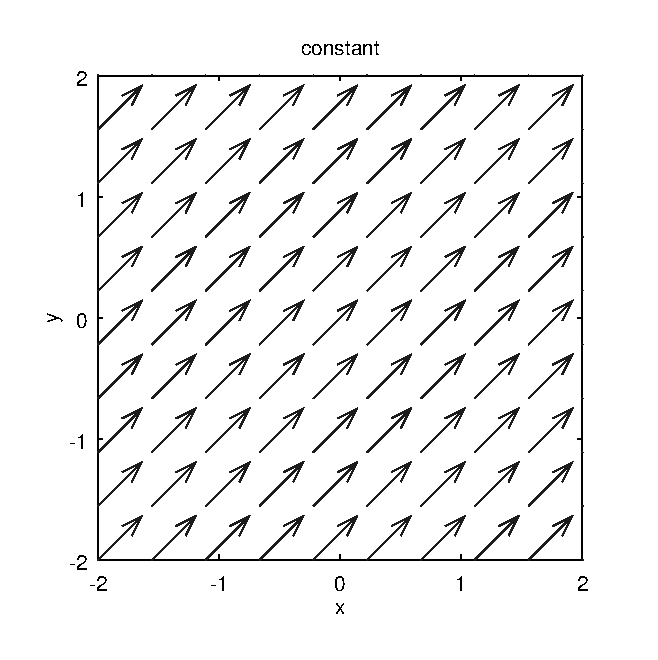
\includegraphics[width=\linewidth]{images/constantflow.eps}
\end{subfigure}
\begin{subfigure}{0.49\linewidth}
\centering
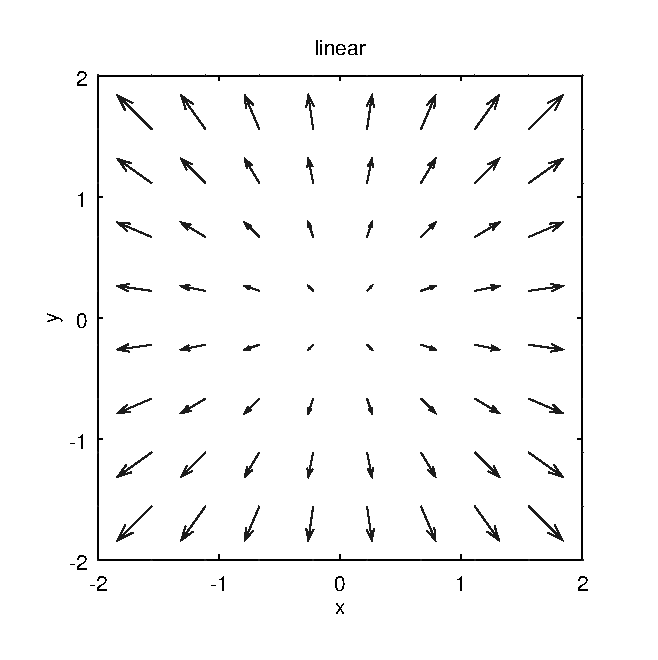
\includegraphics[width=\linewidth]{images/linearflow.eps}
\end{subfigure}
\caption{
Graphs show vector fields of different behaviour, left is constant with $f(x,y) = (1\;\, 1)\T$, right is linear with $f(x,y) = (x \;\, y)\T$.
Constant flow is typical for motion parallel to the image plane, linear flow for motion orthogonal to the image plane. 
}
\label{fig:flowfields}
\end{figure}

Depending on the situation in the image sequence, a constant flow field may be more reasonable than a linear one.
Imagine for example a sequence captured from the view point of a car driver who waits at a crossing while other cars pass the crossing from left to right in front of him.
The optic flow in this situation would be constant as all cars move in the same direction parallel to the image plane.
Now imagine the car driver moving forwards as the crosisng is now free, the whole scene around him will appear to move towards him.
The optic flow is now linear as the surroundings move perpendicular to the image plane.
However, the flow behaviour is not exclusive, both constant and linear flow can be present in the same sequence, for example when another car heading in the same direction switches lanes.
To account for such situations, a variational model has to make more sophisticated assumptions than simple first or second order smoothness.

Fortunately, the presented approach manages to combine first and second order regularisation and even adaptively choose optimal order for a given sequence.
Moreover it provides different adaption shemes to enable a global, local, non-local and region based selection of regularisation.

\section{Variational Model}\label{sec:variationalmodel}
In this section the variational model by Maurer, Stoll and Bruhn introduced in their work \cite{daspaper} will be discussed in detail.
As said in \cref{sec:motivation} the variational model is able to adaptively choose regularization order. 
Therfore the regularisation term is a combination of a first and a second order part.
First the models data term is discussed followed by the first and second order part of the regularization and their underlying concepts.

\subsection{Dataterm}\label{sec:dataterm}
The employed data term in the variational model uses a combination of brightness and gradient constancy assumption.
\begin{flalign}
\label{eq:dataterm}
D(\flow) &= \int_\Omega \charbonnier(p_{\text{brght}}(\flow)) + \gamma*\charbonnier(p_{\text{grad}}(\flow))\;d\x &&
\\\label{eq:brightnessconstancy}
p_{\text{brght}}(\flow) &= (\;I_1(\x+\flow(\x))-I_0(\x)\;)^2 &&
\\\label{eq:gradientconstancy}
p_{\text{grad}}(\flow) &= ||\;\nabla I_1(\x+\flow(\x))-\nabla I_0(\x)\;||_2^2 &&
\end{flalign}
In this setup, $p_{\text{brght}}$ is the penalizer for the brightness constancy assumption and $p_{\text{grad}}$ is the penalizer for the gradient constancy assumption which can be understood as a check for
edges being mapped correctly.
The parameter $\gamma$ is used to weight the terms against each other.
As can be seen $p_{\text{brght}}$ and $p_{\text{grad}}$ are quadratic penalizers, and are thus sensitive to outliers.
To remove the strong influence of outliers on the minimization, the subquadratic charbonnier penalizer \cite{charbonnier} $\charbonnier$ is used to 
robustify both constancy assumptions.
\begin{flalign}\label{eq:charbonnier}
\charbonnier(s^2) &= 2\epsilon^2\sqrt{1+s^2/\epsilon^2} &&
\end{flalign}
Note that the charbonnier penalizer is a function of a squared argument so that an arbitrary quadratically penalized assumption can be plugged in.
When plotting the function with respect to $s$ instead of $s^2$ its behaviour becomes clearer, as shown in \cref{fig:penalizers}.
For values close to zero, the function penalizes quadratically and approaches linear behaviour in the limit $s\to\pm\infty$, resulting in outliers being less fatal.

\subsection{First Order Regularizer}
The first order term of the regularization is the anisotropic complementary regulariser by Zimmer~et~al.~\cite{opticflowinharmony}.
\begin{flalign}
\Rfirst(\flow) &= \int_\Omega S_1(\flow)\;d\x&&
\\\label{eq:S1}
S_1(\flow) &= \peronamalik\Big((\ev_1\T\nabla u)^2+(\ev_1\T\nabla v)^2\Big)
+ \charbonnier\Big((\ev_2\T\nabla u)^2+(\ev_2\T\nabla v)^2\Big)&&
\end{flalign} 
This term makes use of the eigenvectors of the regularisation tensor \cite{opticflowinharmony}.
The regularization tensor is a generalization of the structure tensor \cite{maxanisotropy} for arbitrary image features.
In short, it summarizes gradient information within a neighborhood of a pixel.
The eigenvector $\ev_1$ points in the direction of steepest change (i.e. over an edge) while $\ev_2$ is orthogonal to $\ev_1$ (i.e. points along an edge).

Lets postpone the discussion of the regularization tensor for a second and get some intuition on the way $S_1$ works.
As can be seen from \cref{eq:S1}, the term uses two penalizer functions, the Charbonnier penalizer which was introduced in \cref{sec:dataterm} in \cref{eq:charbonnier} and the Perona~Malik penalizer $\peronamalik$.
\begin{flalign}\label{eq:peronamalik}
\peronamalik(s^2) &= \epsilon^2\ln(1+s^2/\epsilon^2)&&
\end{flalign}
As arguments to the penalizer functions, projections of the flow gradients onto the eigenvectors are used.
These projections are minimal if the flow gradient vanishes as in standard first order smoothness terms.
Special about this term are the different penalizations of projections on the first and second eigenvector respectively.
The graphs of the two penalizer functions are shown in \cref{fig:penalizers}, where it can be seen that values close
to zero are penalized quadratically, values further away are penalized subquadratically in both functions.
In the limit however, the Perona-Malik penalizer takes on smaller values than the charbonnier penalizer.
This has the effect of flow changes tangent to the first eigenvector to be less costly than tangent to the second eigenvector.
From the perspective of image features and the regularization tensor this is like getting a \enquote{discount} on flow change over an edge.
\begin{figure}[htb]
\centering
\begin{subfigure}{0.49\linewidth}
\centering
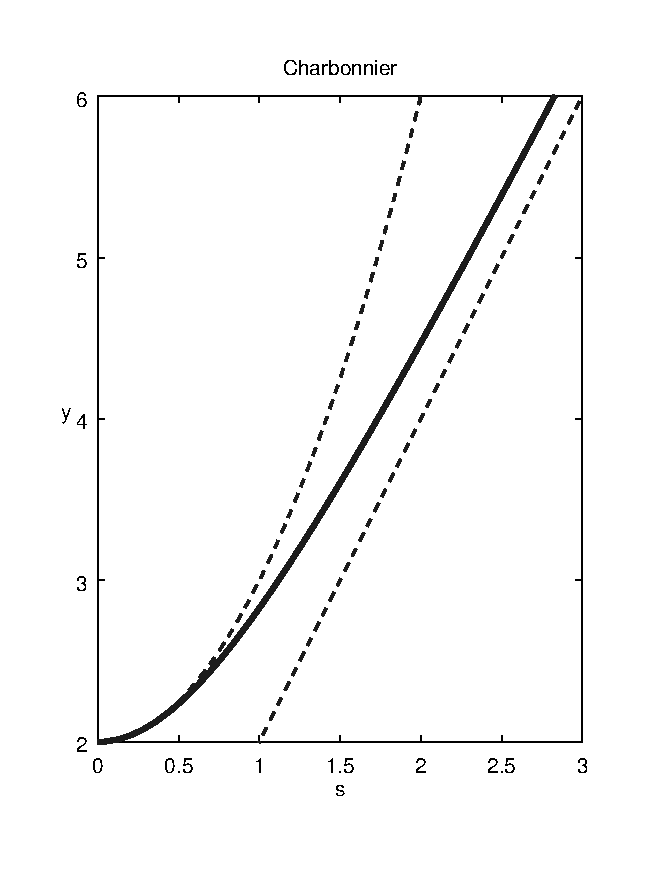
\includegraphics[width=\linewidth]{images/charbonnier.eps}
\end{subfigure}
\begin{subfigure}{0.49\linewidth}
\centering
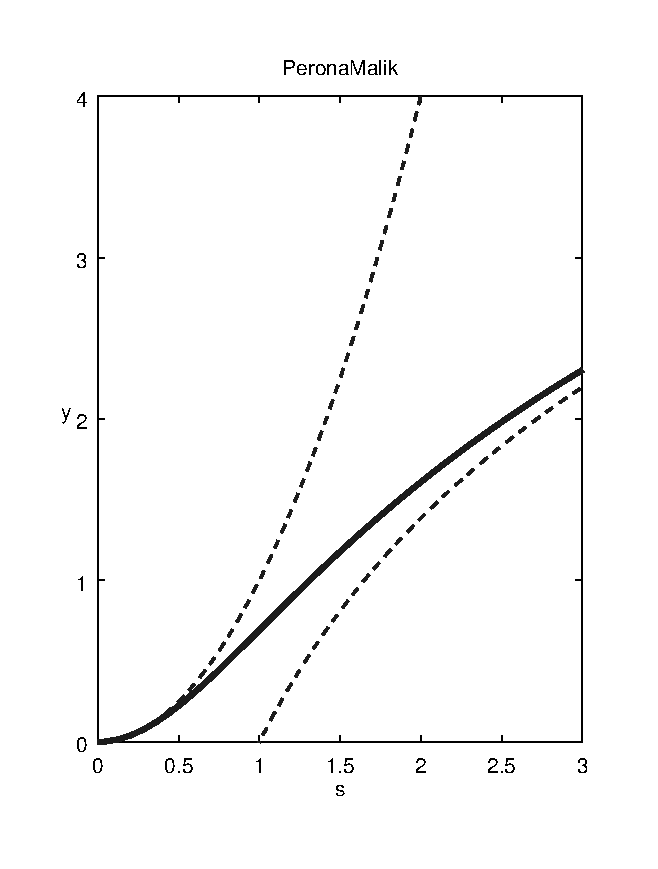
\includegraphics[width=\linewidth]{images/peronamalik.eps}
\end{subfigure}
\caption{
Graphs show penalizer functions and their asymptotic equivalents as dashed lines.\\
Left is charbonnier \cref{eq:charbonnier} with $\epsilon=1$ and asymptotic equivalents $\lim_{s\to 0}\charbonnier(s^2)=s^2+2$ and $\lim_{s\to\infty}\charbonnier(s^2)=2s$.\\
Right is Perona Malik \cref{eq:peronamalik} with $\epsilon=1$ and asymptotic equivalents $\lim_{s\to 0}\peronamalik(s^2)=s^2$ and $\lim_{s\to\infty}\peronamalik(s^2)=2\ln(s)$.
}
\label{fig:penalizers}
\end{figure}

\subsubsection{Regularization Tensor}
To continue the discussion of the regularization tensor, lets state its definition first.
\begin{flalign}\label{eq:structuretensor}
\mathcal{S}_{\Phi,\omega}(\x) &= \bigintsss \omega(\tau)\Mat{\Phi_x(\x-\tau)^2 & \Phi_x(\x-\tau)\Phi_y(\x-\tau)\\\Phi_x(\x-\tau)\Phi_y(\x-\tau) & \Phi_y(\x-\tau)^2} \;d\tau
&&\\\label{eq:eigendecomp}
\mathcal{S}_{\Phi,\omega}&= Q \Lambda Q\T = \mat{\ev_1&\ev_2}\mat{\lam_1&0\\0&\lam_2}\mat{\ev_1\T\\ \ev_2\T}&&
\end{flalign}
The tensor is a convolution of a weighting function $\omega$ with a matrix.
The matrix is the outer product of the gradient of the selected image feature $\Phi$ which is calculated as $\nabla\Phi(\x)\nabla\Phi(\x)\T$.
For the structure tensor the image feature would be brightness $\Phi=I$, but as this is the generalization, $\Phi$ can be something else like the saturation value in HSV color space or luminance of CIE L*a*b*.
Typically, the feature is chosen to be consistent with the feature used in the data term, which would be a combination of brightness and gradient norm.
Using the eigendecomposition (\cref{eq:eigendecomp}), the orthonormal eigenvectors $\ev_1$ and $\ev_2$ are obtained which summarize the gradient distribution in the neighborhood defined by the weighting function $\omega$.
If the weighting function was a Dirac delta $\omega = \delta$ the eigendecomposition of the tensor would yield the normalized gradient as first eigenvector.
\begin{flalign*}
\mathcal{S}_{\Phi,\delta}= \nabla\Phi\nabla\Phi\T = \lambda_1*\ev_1\ev_1\T = \mat{\ev_1&\ev_2}\mat{\lambda_1&0\\0&0}\mat{\ev_1\T\\ \ev_2\T}&&
\end{flalign*}
Here the first eigenvalue is the squared length of the gradient $\lambda_1=|\nabla\Phi|^2$.
Of course this discussion only holds for Dirac delta as weighting function, for others like Gaussian, the eigenvectors cannot be factored in this way.

\subsection{Second Order Regularizer}\label{subsec:secondorderreg}
The second order regularizer makes use of two auxiliary functions $\aaux(\x)$ and $\baux(\x)$ which are connected
to the flow $\flow$ using a coupling term $S_2$. 
These auxiliary functions are as well unknown and are controlled by an auxiliary smoothness term $S_\text{aux}$.
\begin{flalign}
\Rsecond(\flow) =\;&\int_\Omega\; \inf_{\aaux,\baux}\big[\;S_2(\flow,\aaux,\baux) +\beta*S_\text{aux}(\aaux,\baux)\;\big] \;d\x
&&\\
S_2(\flow,\aaux,\baux) =\;& \peronamalik\Big( (\ev_1\T(\nabla u-\aaux))^2 + (\ev_1\T(\nabla v-\baux))^2 \Big)
&&\\
+\;&\charbonnier\Big( (\ev_2\T(\nabla u-\aaux))^2 + (\ev_2\T(\nabla v-\baux))^2 \Big)
\nonumber&&\\
S_\text{aux}(\aaux,\baux) =\;& \peronamalik\Big(\sum\nolimits_{k=1}^2\;(\ev_k\T \jacob_{\aaux}\;\ev_1)^2 + (\ev_k\T \jacob_{\baux}\;\ev_1)^2  \Big)
&&\\
+\;&\charbonnier\Big(\sum\nolimits_{k=1}^2\;(\ev_k\T \jacob_{\aaux}\;\ev_2)^2 + (\ev_k\T \jacob_{\baux}\;\ev_2)^2  \Big)
\nonumber&&
\end{flalign}
This regularization term can be interpreted as the integral over the infimal convolution of $S_2$ and $S_\text{aux}$ with respect to the vector fields $\aaux$ and $\baux$.

The coupling term $S_2$ is similar to the first order term $S_1$ in that it uses the two penalizer functions $\peronamalik$ and $\charbonnier$ to penalize non zero projections with respect to the eigenvectors of the structure tensor (\cref{eq:structuretensor}).
This time however, not the flow gradients themselves are projected, but the differece of the gradients to the auxiliary functions.
The coupling term therefore becomes minimal if the gradients are euqal to the auxiliary functions instead of equal to zero as in the first order term.
Again, the prejection on the first eigenvector is penalized less due to the behavior of the perona malik penalizer, but is not intuitive in the form written above.
If instead we reformulate the projection as $(\ev_1\T(\nabla u-\aaux))^2 = (\ev_1\T\nabla u-\ev_1\T\aaux)^2$ it becomes clear that the flow gradient and the auxiliary function are allowed to differ as long as they are roughly tangent to the first eigenvector.

In the auxiliary term $S_\text{aux}$ the Jacobians of the auxiliary functions $\jacob_{\aaux}$ and $\jacob_{\baux}$ are anisotropically penalized similar to the first order penalization of the flow gradients.
Obviously, the auxiliary term is minimal if the derivatives of the auxiliary functions vanish, allowing for constant auxiliary functions with changes at edges which are indicated by the regularization tensor.
Due to the connection of the auxiliary functions to the flow gradients in the coupling term, the flow is indirectly constrained to be linear.
This is because the nullspace of the second order term are functions with derivatives equal to the auxiliary functions which are constrained to be constant.

\section{Order Adaption}
In \cref{sec:variationalmodel}, the data and regularization terms were discussed and it was explained that the first order regularizer enforces constant flow whereas the second order regularizer allows for linear flow.
As illustrated in \cref{fig:flowfields} constant vector fields are suitable for modelling motion parallel to the image plane, motion orthogonal to the image plane can be modelled using a linear flow field.
So what is needed to apply the most suitable regularizer depending on the current sequence, is an adaptive scheme.
In the following four different schemes will be discussed, where the global scheme will be used to introduce the underlying concept of the schemes.

\subsection{Global Scheme}
The global adaptive scheme will be choosing order once for the whole image domain.
To do so a general regularization term consisting of both, first and second order, will be extended.
The general regularization term is a simple convex combination of the terms with weighting parameter $c\in [0,1]$ and selecton term $\phi_\lambda(c)$ of the following form.
\begin{flalign}
R(\flow,c) = \int_\Omega \inf_{\aaux,\baux}\big[\; c*S_1(\flow) 
& + (1-c)*S_2(\flow,\aaux,\baux) 
&&\\
& + \beta*S_\text{aux}(\aaux,\baux)
+ \phi_\lambda(c)\;\big] \;d\x \nonumber&&
\end{flalign}
It may be counter intuitive to only include $S_1$ and $S_2$ in the convex combination and not $S_\text{aux}$, but $S_\text{aux}$ is independent of $\flow$ and merely used to constrain the auxiliary functions.
$S_1$ and $S_2$ on the other hand are the energies with respect to the flow and are comparable to each other as they only differ in the projected quantity, which was already discussed in \cref{subsec:secondorderreg}.
The goal thus, is to embed some information into the the weighting parameter $c$ such that it equals to $1$ when first order regularization has less energy than second order regularization and equals to $0$ in the contrary case.
However, since the class of linear functions which can be modelled using second order regularization includes constant functions, it is only desirable to use second order regularization when it yields a significant benefit over first order.
To model this behavour of $c$ a sigmoid function of the benefit $\Delta$ of first over second order regularization is used as illustrated in \cref{fig:c_phi}.
\begin{flalign}\label{eq:c}
c = \frac{1}{1+e^{-\Delta/\lambda}} \quad\text{with}\quad\Delta=T+\frac{1}{|\Omega|}\int_\Omega S_2 - S_1 \; d\x &&
\end{flalign}
Here $\lambda$ is used to control the slope of the sigmoid function, and $T$ is the threshold by which the second order regularizer has to be better than first order, so that second order will be used.

To get to this behavior of $c$ from the euler lagrange equation's point of view, the corresponding selection term $\phi_\lambda(c)$ has to be found.
By examining the regularizers partial derivative $\frac{\partial R}{\partial c} = 0$ we get to the following equation.
\begin{flalign}
\frac{\partial R(\flow,c)}{\partial c} = &\int_\Omega S_1(\flow) - S_2(\flow,\aaux,\baux) + \phi_\lambda'(c) \;d\x \;=\; 0
&&\nonumber\\
-\phi_\lambda'(c)*|\Omega| = &\int_\Omega S_1(\flow) - S_2(\flow,\aaux,\baux) \;d\x
&&\nonumber\\
\label{eq:deriv_r_to_c}
\phi_\lambda'(c) = \frac{1}{|\Omega|}&\int_\Omega S_2(\flow,\aaux,\baux) - S_1(\flow) \;d\x
&&
\end{flalign}
The right hand side of \cref{eq:deriv_r_to_c} also occurs in \cref{eq:c} which can be reformulated as follows in order to be plugged in.
\begin{flalign}
&\frac{1}{|\Omega|}\int_\Omega S_2 - S_1\;d\x = \Delta-T
%&&\nonumber\\
\quad\text{with}\quad
\Delta = -\lambda*\ln(\frac{1}{c}-1)
&&\nonumber\\\label{eq:phi'}
&\phi_\lambda'(c) = -\lambda*\ln\Big(\frac{1}{c}-1\Big) - T
\end{flalign}
To obtain $\phi_\lambda$ we integrate both sides of \cref{eq:phi'} and get the following selection term with integration constant $C$.
\begin{flalign}
\phi_\lambda(c) = \lambda \Bigg( \ln(1-c)-c*\ln\Big(\frac{1}{c}-1\Big) \Bigg) -Tc + C &&
\end{flalign}
When chosing $C=T$ we can get a more intuitive formulation of the regularizer, using a cleverly tailored replacement $\phi$ for $\phi_\lambda$.
\begin{flalign}\label{eq:phi}
\phi(c) = \frac{\phi_\lambda(c) + T*(c-1)}{\lambda} &= \ln(1-c)-c*\ln\Big(\frac{1}{c}-1\Big)
&&\\
%= \ln(1-c)-c*\ln\Big(\frac{1-c}{c}\Big) 
& = c*\ln(c) + (1-c)*\ln(1-c)
%-c ln(1/c -1 ) = -c ln((1-c)/c) = -c ln(1-c) + c ln(c)
&&\nonumber\\
R(\flow,c) = \int_\Omega \inf_{\aaux,\baux}\big[\; c*S_1(\flow) 
& + (1-c)*\big(S_2(\flow,\aaux,\baux) +T\big)
&&\\
& + \beta*S_\text{aux}(\aaux,\baux)
+ \lambda*\phi(c)\;\big] \;d\x \nonumber&&
\end{flalign} 
In this representation the threshold parameter $T$ appears in the convex combination together with $S_2$ and can be interpreted as an extra cost to be paid in order to use second order regularization.
The sigmoid slope parameter $\lambda$ now works as a weight for the selection term $\phi$ which has become independent of $\lambda$.
In fact the selection term has simplified quite a bit and it can be seen that it is a symmetric function which is illustarted in \cref{fig:c_phi}.
From the figure it can also be seen that $\phi$ is minimal for $c=\frac{1}{2}$ which can be interpreted as a prior on $c$ for when the model is indecisive on regularization order.
So by definition of $\phi$ neither of the regularizers is preferred, but due to the threshold $T$ the descision is biased towards the first order regularization.

\begin{figure}[htb]
\centering
\begin{subfigure}{0.49\linewidth}
\centering
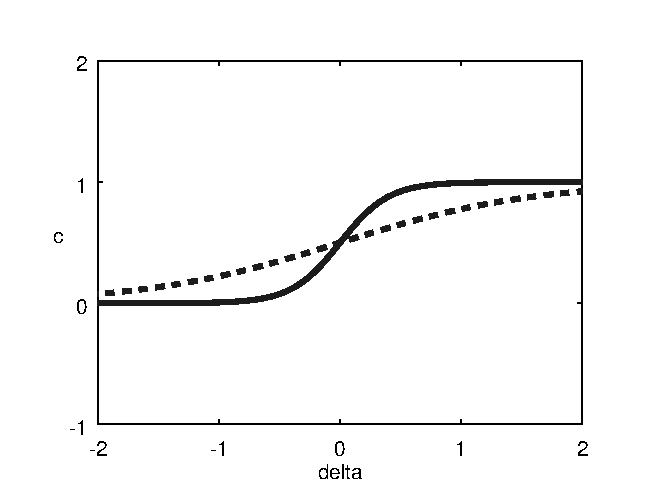
\includegraphics[width=\linewidth]{images/cofdelta.eps}
\end{subfigure}
\begin{subfigure}{0.49\linewidth}
\centering
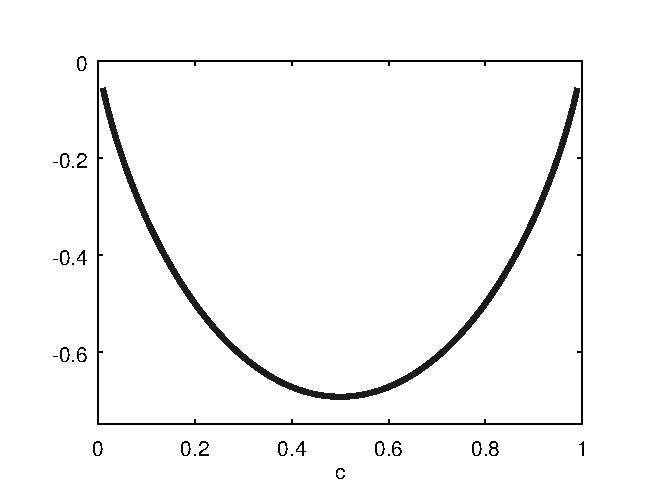
\includegraphics[width=\linewidth]{images/selectionterm.eps}
\end{subfigure}
\caption{
The left graph shows the weighting parameter $c$ (\cref{eq:c}) with respect to $\Delta$, where $\Delta$ is the benefit of first over second order regularization biased by the threshold $T$.
The solid line corresponds to $\lambda=0.2$, the dotted line to $\lambda=0.8$.
\\
The right graph shows the selection term $\phi(c)$ (\cref{eq:phi}) which is axially symmetric to $c=\frac{1}{2}$.
}
\label{fig:c_phi}
\end{figure}

\subsection{Local Scheme}
The previously introduced global scheme chooses regularization for the whole image domain, however, different parts of the scene may move differently so that it makes sense to
allow for different regularization depending on the location.
So instead of using a global weighting parameter $c$, it is replaced by a weighting function $c_{\text{local}}(\x)$.
\begin{flalign}
c_{\text{local}}(\x) = \frac{1}{1+e^{-\Delta(\x)/\lambda}} \quad\text{with}\quad\Delta(\x)=T + S_2 - S_1&&
\end{flalign}
As a consequence $\Delta$ is now a spacially varying function as well, mapping to the benefit of first order regularization in a single pixel at $\x$, which allows the model to decide on order on a per pixel basis.

\subsection{Non-Local Scheme}
Since the local scheme allows for different regularization order per pixel based on a decision which only takes that pixels location into account, regularization order may fluctuate a lot in this model.
To make the descision more consistent with the pixels neighorhood, the weighting function $c_{\text{local}}(\x)$ is altered to
take a rectangular shaped patch of pixels around it into account.
\begin{flalign}
\cNl(\x) = \frac{1}{|\patch(\x)|}\int_{\patch(\x)}\cnl(\y)\;d\y 
&&\\
R_\text{nl}(\flow,\cnl) = \int_\Omega \inf_{\aaux,\baux}\big[\; \cNl*S_1(\flow) 
& + (1-\cNl)*\big(S_2(\flow,\aaux,\baux) +T\big)
&&\\
& + \beta*S_\text{aux}(\aaux,\baux)
+ \lambda*\phi(\cnl)\;\big] \;d\x \nonumber&&
\end{flalign}
Here $\mathcal{N}(\x)$ denotes the patch of $\x$ and $|\mathcal{N}(\x)|$ the patch size which is used for normalization.
To find $\cnl$, $R_\text{nl}(\flow,\cnl)$ is minimized with respect to it and yields:
\begin{flalign}
\cnl(\y) = \frac{1}{1+e^{\Delta(\y)/\lambda}} \quad\text{with}\quad \Delta(\y) = \int_{\mathcal{N}(\y)} \frac{ T + S_2 - S_1 }{|\mathcal{N}(\x)|} \;d\x
&&
\end{flalign}
It may be surprising at first that the integrated $\cnl$ itself contains a nested integral, but it is easy to convince yourself when thinking about a 
discrete version $c_{\x}$.
When taking the derivative with respect to a single $c_{\x}$, then due to the integral in $\cNl$ we need to identify all terms which contain $c_{\x}$ (which is defined by the patch $\mathcal{N}(\x)$).
The reason for normalization $\frac{1}{|\mathcal N(\x) |}$ being inside the integral is that patches at the boundaries vary in size (become smaller as less pixels are defined there).

\subsection{Region-Based Scheme}
The non-local scheme takes a neighborhood around a pixel into account for the descision on regularization order.
To push it yet a little further, the region based scheme decides on order leveraging a level-set function $z(\x):\Omega\to\mathbb{R}$ which devides the image space into first and second order regularized regions.
Recall that a level-set function defines a closed curve (or curves) by $\{\x \;|\; z(\x)=0\}$ that defines the descision boundary.
The regions are thus defined by $\{\x \;|\; z(\x) < 0\}$ and $\{\x \;|\; z(\x) > 0\}$ which will be leveraged to regionally decide on regularization order.
The corresponding regularizer reads as follows.
\begin{flalign}
&R(\flow,z) = \int_\Omega c_\text{rgn}(z)*S_1 + (1-c_\text{rgn}(z))*(S_2 + T) + \theta*|\nabla c_\text{rgn}(z)| \;d\x
&&\\
&c_\text{rgn}(z) = \frac{1}{1+e^{z/\lambda}}
&&
\end{flalign}
Here $c_\text{rgn}$ is as well a sigmoid function, but choosen to approximate the heaviside funtion ($\lambda\to 0$) in order to obtain hard boundaries for the regions defined by $z$.
The selection term from the previous schemes has been replaced by a smoothness term on $c_\text{rgn}$ which penalizes non-smooth level set functions which results in less sign changes.
Due to this penalization short paths for $\{\x \;|\; z(\x)=0\}$ are favored resulting in smooth region boundaries.

Unfortunately this sophisticated scheme comes at a larger computational cost as $z$ has to be evolved due to its smoothenss term \cite{someone}.


\section{Experiments}
To evaluate this new approach, the authors conducted a few experiments which will be presented in this section.

To get an insight into the order selection of the algorithm with the different selection schemes, four synthetic image sequences were created from which the actual flow fields could be extracted as ground truth.
\Cref{fig:classroom} shows the 4 image pairs and their corresponding flow fields.

\begin{figure*}[htb]
\centering
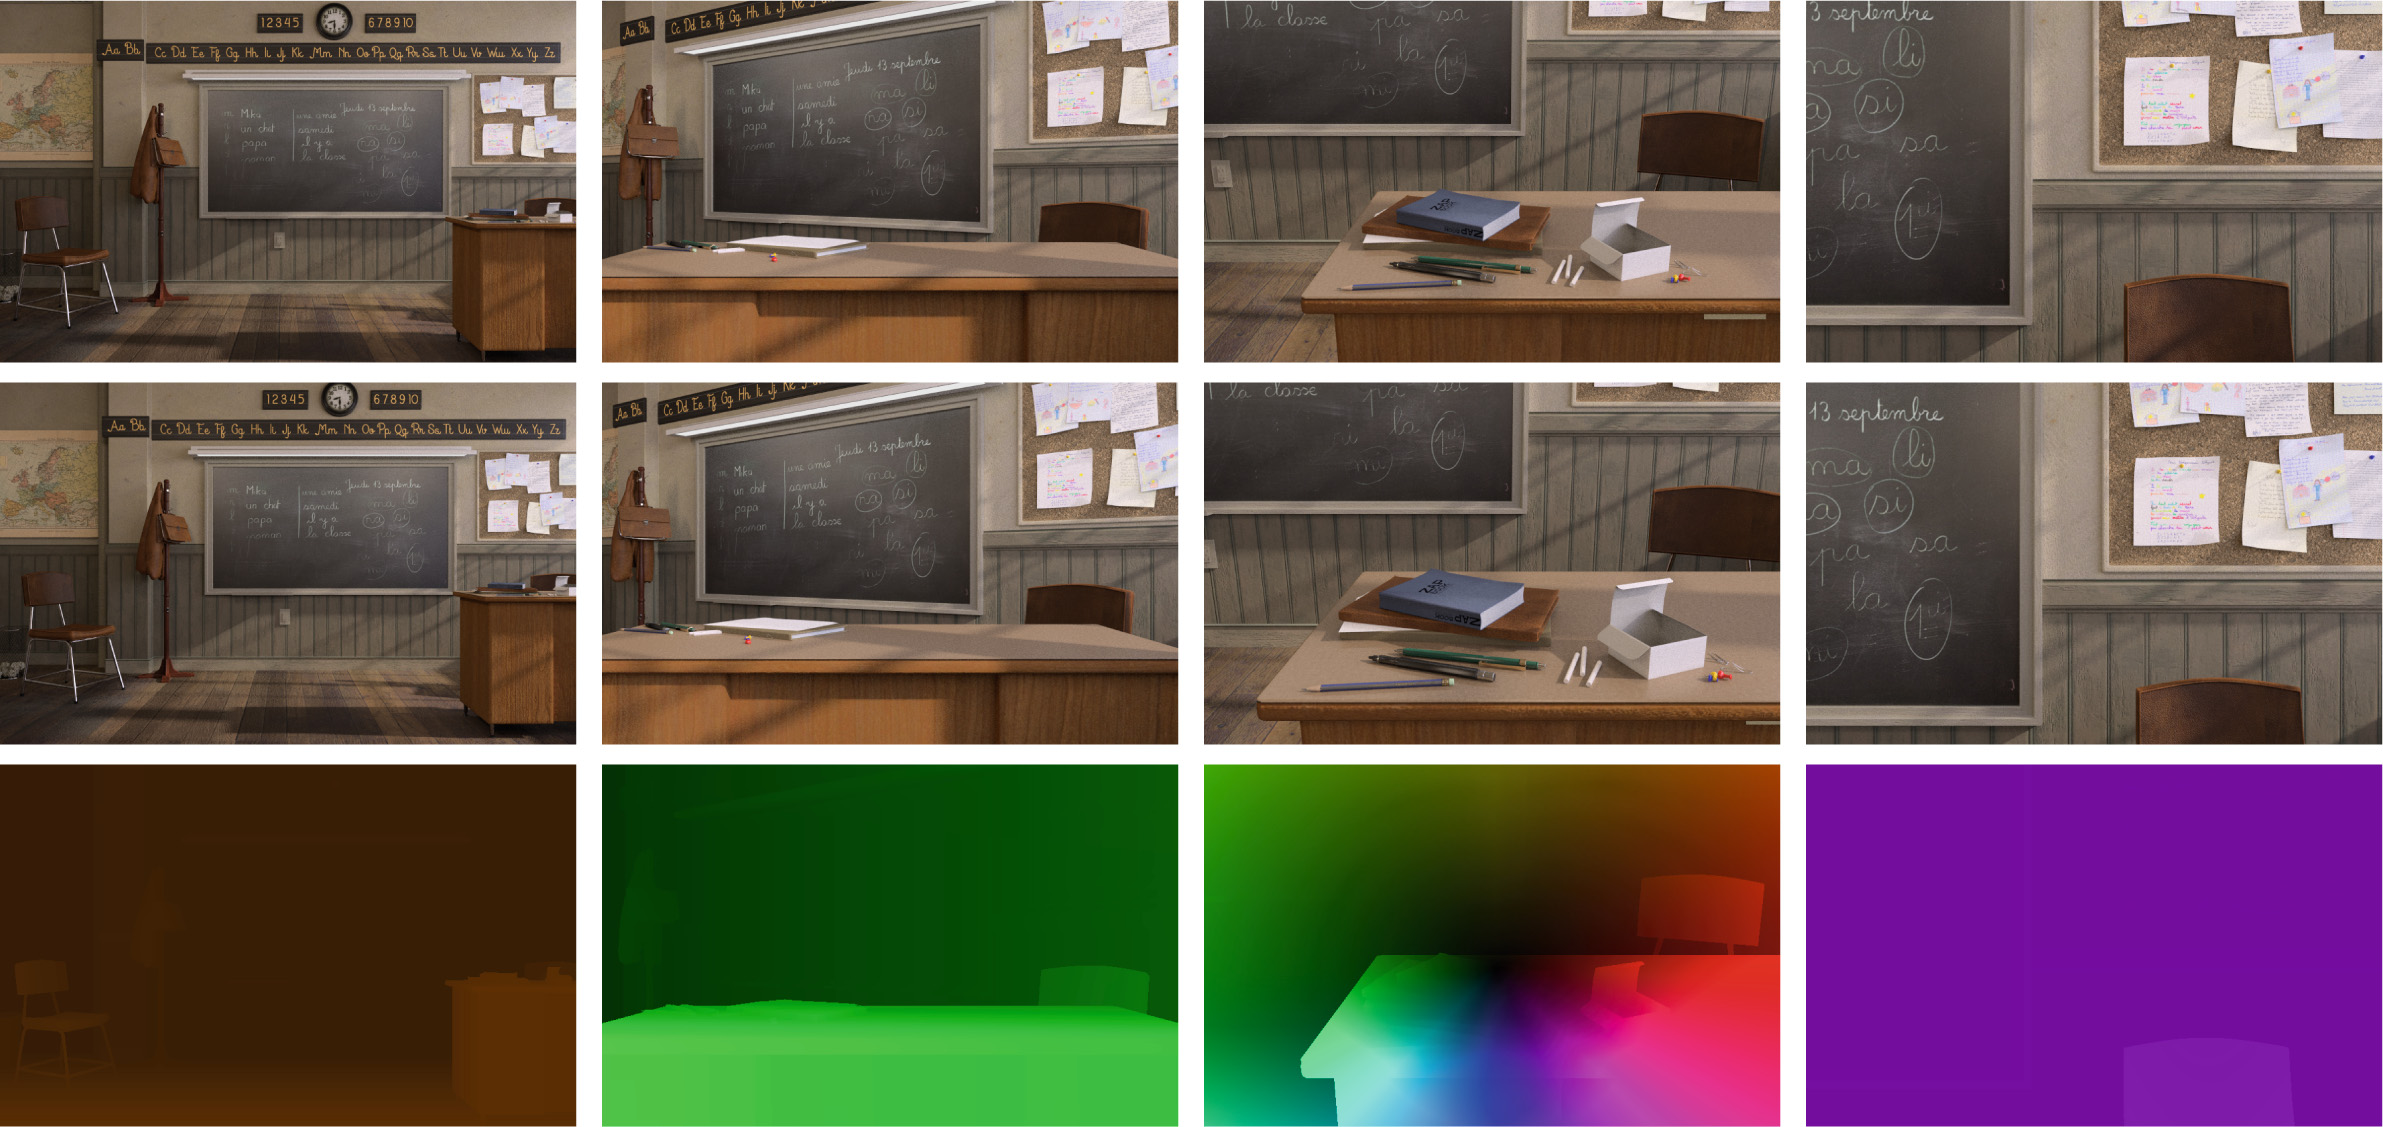
\includegraphics[width=0.9\linewidth]{images/classroom.png}
\caption{\textbf{Classroom sequences}~\cite{daspaper}. 
First and second rows contains first frames and second frames.
Third row contains the corresponding flow fields with flow direction encoded by hue, and flow magnitude by brightness.
Each column corresponds to another sequence.
Sequences 1,2 and 4 result from fronto-parallel motion as can be seen from the flow directions being the same for each pixel.
Sequence 3 results from \enquote{fronto-orthogonal} or affine motion similar to the linear flow field depicted in \cref{fig:flowfields}.}
\label{fig:classroom}
\end{figure*}

By looking at the gradient magnitude $\big|\deriv{\flow(\x)}{\x}\big|$ of the ground truth flow field, areas of vanishing gradients can be identified.
Small values of the gradient magnitude thus indicate fronto-parallel motion whereas large values indicate affine motion.
When these are compared to the order deciding $c$ term of the different schemes, we can get a good impression on how the algorithm decided.

\begin{figure*}[htb]
\centering
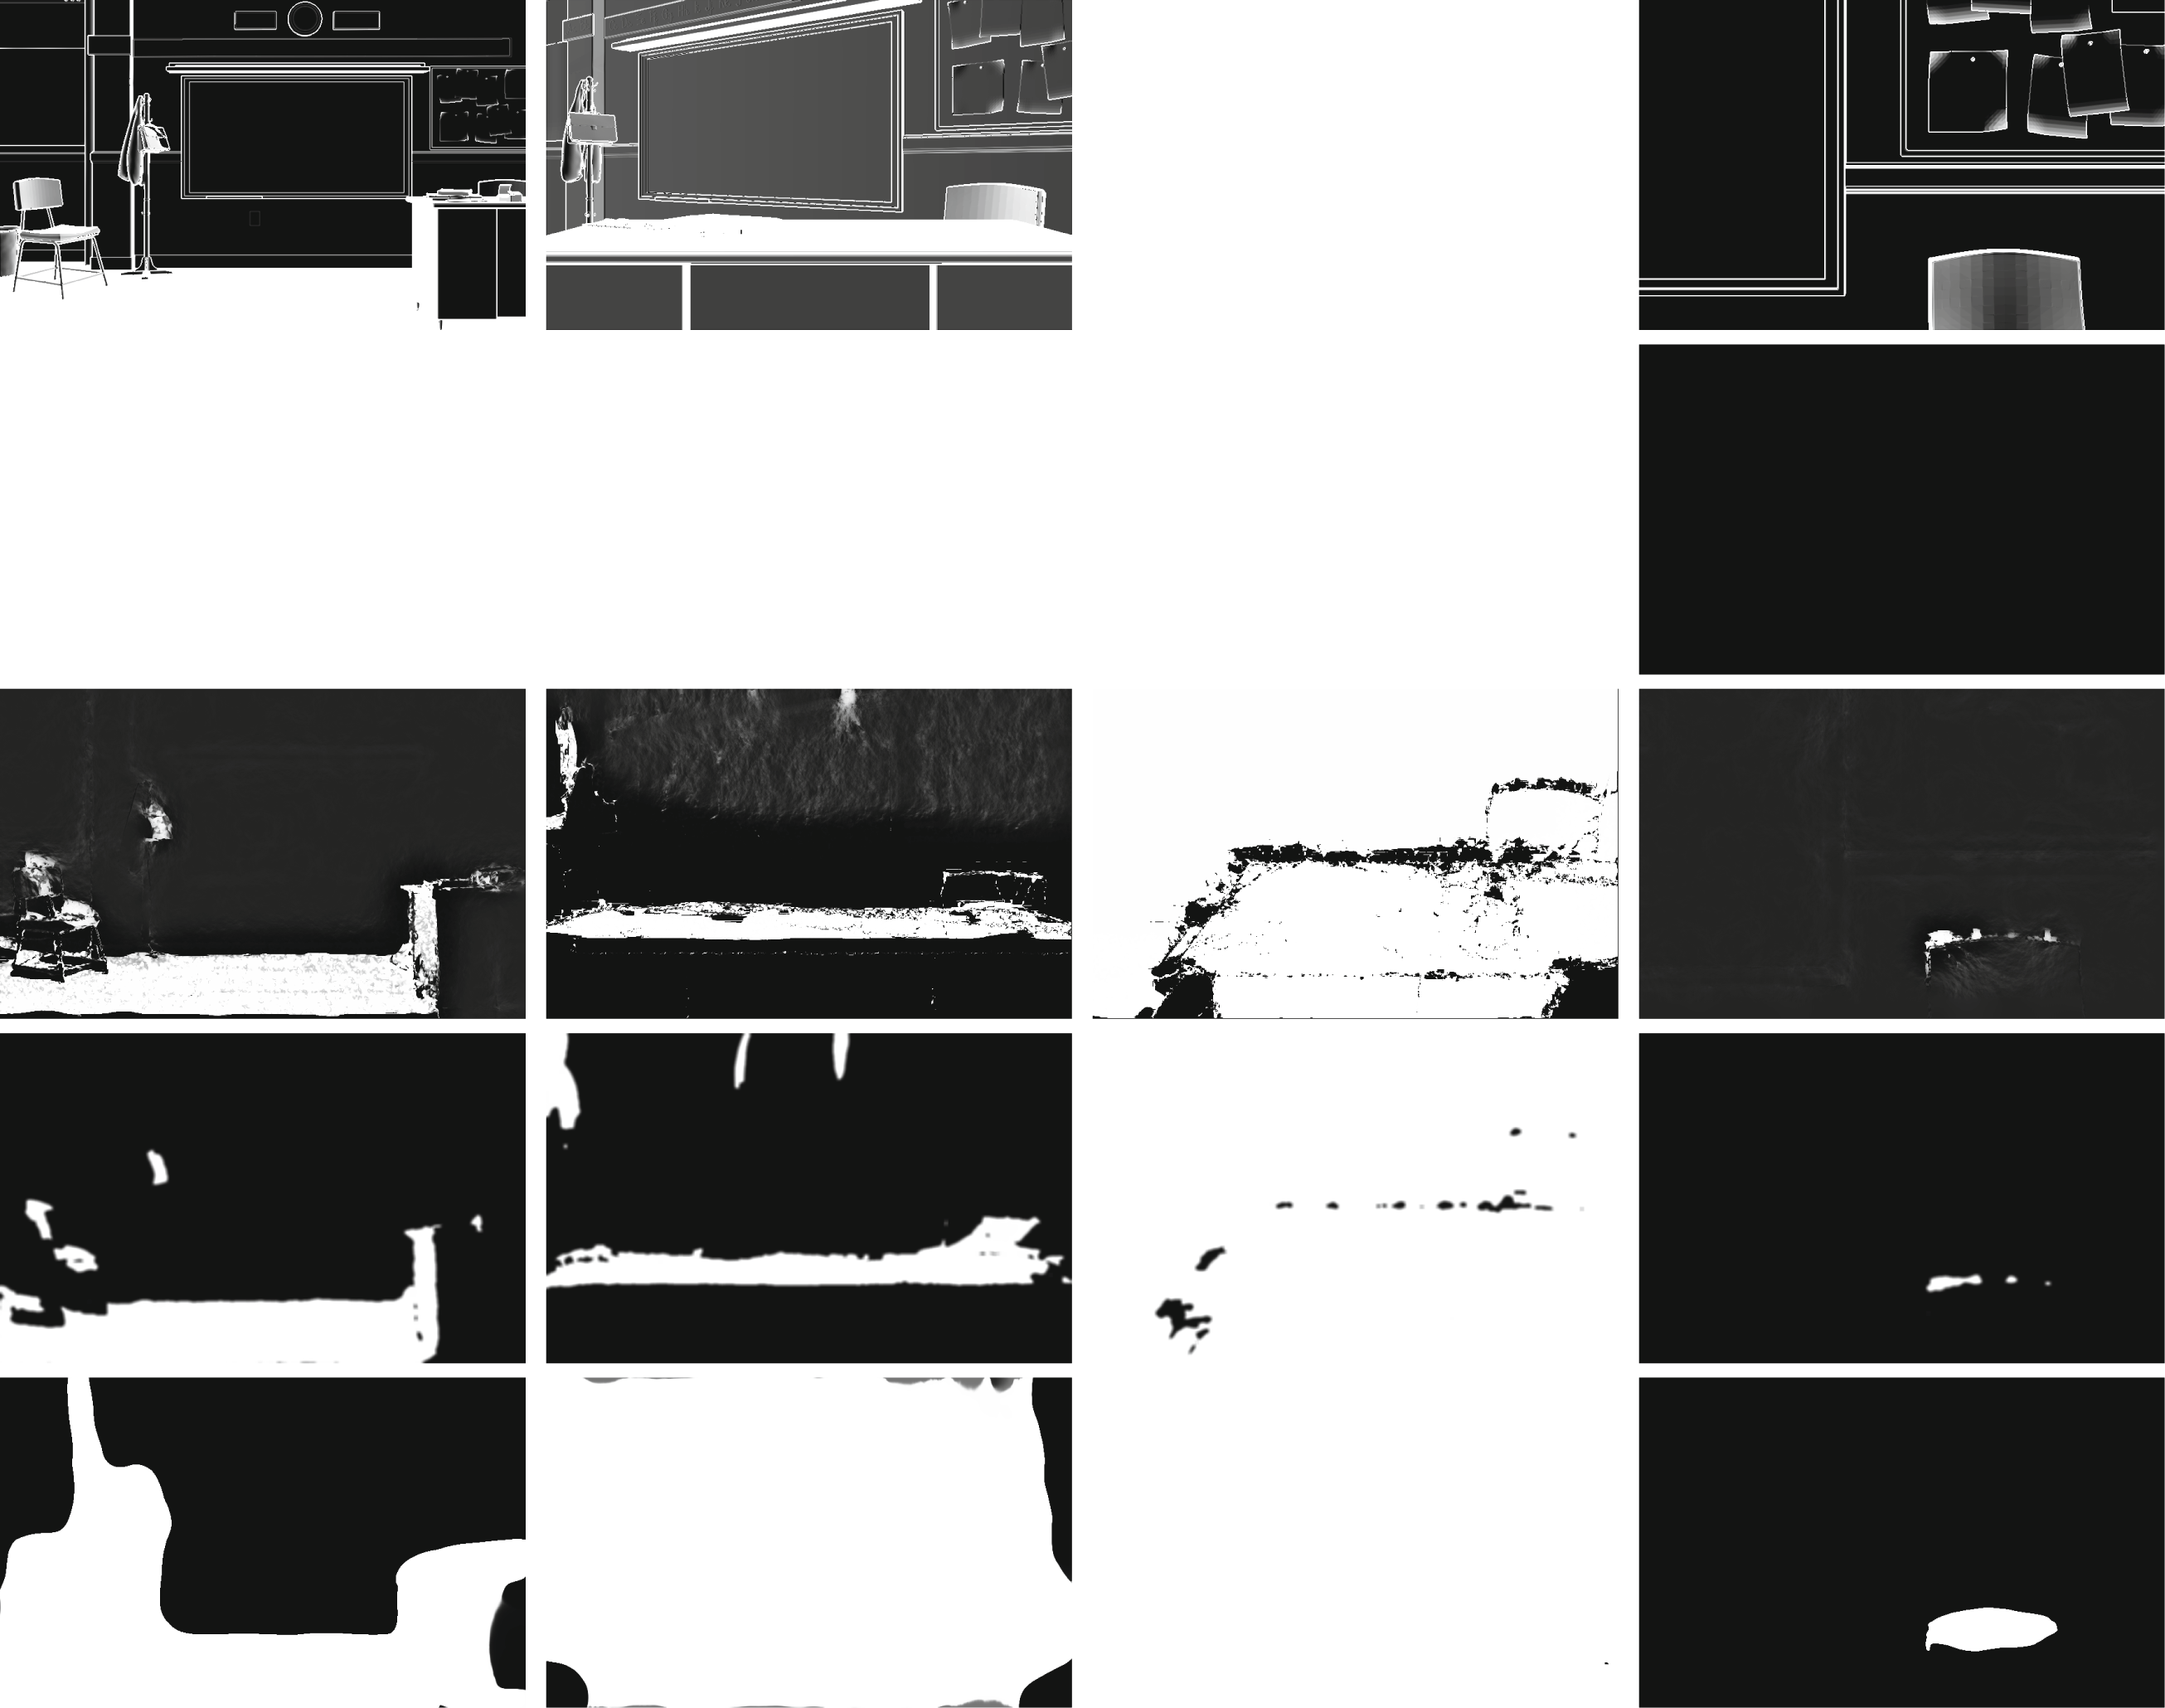
\includegraphics[width=0.9\linewidth]{images/classroom_c.png}
\caption{Adaption behavior of the different schemes~\cite{daspaper}. 
Each column corresponds to the respective sequence introduced in \cref{fig:classroom}.
First row shows the gradient magnitude of the ground truth flow fields, dark pixels indicate small magnitudes,
bright pixels high magnitudes.
The following rows correspond to the regularization order selection parameters $c$, dark pixels indicate first order regularization, bright pixels indicate second order regularization.
The second row corresponds to the global scheme, third to local, fourth to non-local and fifth to region based. 
}
\label{fig:classroom_c}
\end{figure*}

\Cref{fig:classroom_c} shows a comparison of the adaption behavior of the four different adaption schemes with respect to the ground truth gradient magnitude which works as an indicator for regularization order.
For the global scheme (2nd row) the images are either completely white or completely black as the selection is global and thus the same for each pixel.
For the global scheme, the algorithm surprisingly picked second order regularization for all sequences except for the fourth sequence.
On the other hand, the fourth sequence has almost no depth to it and is thus truly fronto-parallel, so all schemes decided for first order for the majority of the pixels.
What can also be seen is that for the local scheme (third row) the selection is pretty noisy, whereas the non-local and region based scheme show way more consistent order selection.
Another insight is, that at motion discontinuities (i.e. edges) first order regularization is chosen predominantely.
Finally it is important to note that different order selection than indicated by the ground truth does not necessarily imply a bad result, since second order regularization contains first order as previously explained.

The quality of the approach has not only been aseesed visually, but also quantitatively by evaluating the average end point error (AEE).
The four regularizers (global , local, non-local, region) therefore were put up against a purely first and purely second order regularizer on the class room sequences.
The second order regularizer used for comparison is an anisotropic variant of total generalized variation (TGV~\cite{tgv}) which also uses a coupling term and is not a purposefully chosen inferior regularizer.  
The AEE results for the different sequences are shown in \cref{tbl:classroom_aee}.
From the table it can be seen that the best results are found in the order adaptive segment except for the fourth sequence where the first order regularizer shares first place with the adaptive local regularizer.
Also the second order regularizer is already outperformed by the global order adaptive regularizer.
For the rather fronto-parallel sequences, the local adaptive regularizer shines, but has really poor performance on the third sequence which is heavily affine in motion.
The non-local and region order adaptive regularizers on the other hand, do quite well in all of the sequences, the region order adaptive however performs best on the affine motion sequence.
Also note that the global order adaptive regularizer does not simply amount to choose best out of first and second order, but instead relies on the same hyperparamters as the other adaptive regularizers (which were optimized jointly).
Due to the number variables to be evolved in order to approximate the flow ($\flow, \aaux, \baux, c$) the runtimes of the adaptive regularizers are quite high compared to the simple first order regularizer which does not have a coupling term (and thus no auxiliary functions), especially the the region adaptive order regularizer takes quite a while as it involves the evolution of a smooth level set function.  

\begin{table}[htb]
%% Table captions on top in journal version
\caption{\label{tbl:classroom_aee} Average endpoint error - Classroom sequences~\cite{daspaper}}
\scriptsize
\begin{center}
\begin{tabular}{r|cccc|c}
regularization & Seq. 1 & Seq. 2 & Seq. 3 & Seq. 4 & runtime 
\\\hline
first order        & 0.129 & 0.358 & 2.038 & \textbf{0.088} & 17s
\\
second order       & 0.141 & 0.370 & 0.669 & 0.102 & 75s
\\\hline
adaptive global    & 0.141 & 0.365 & 0.667 & 0.095 & 100s
\\
adaptive local     & \textbf{0.111} & \textbf{0.260} & 1.115 & \textbf{0.088} & 105s
\\
adaptive non-local & 0.116 & 0.275 & 0.737 & 0.095 & 120s
\\
adaptive region    & 0.125 & 0.366 & \textbf{0.662} & 0.098 & 180s
\end{tabular}
\end{center}
\end{table}

Of course the results on the self made image sequences are not easily put into perspective with other recent approaches regarding optic flow, which is why the authors also put the regularizers up against the Middlebury benchmark~\cite{middlebury}, the Sintel benchmark~\cite{sintel} and the KITTI benchmarks of 2012~\cite{kitti12} and 2015~\cite{kitti15}.


\begin{table}[htb]
%% Table captions on top in journal version
\caption{\label{tbl:benchmarks} Average endpoint error (AEE) and bad pixel error (BP) in four different benchmarks~\cite{daspaper}}
\scriptsize
\begin{center}
\begin{tabular}{r|cccc}
regularization & Middlebury & Sintel & KITTI '12 & KITTI '15
\\
& (AEE) & (AEE) & (BP) & (BP)
\\\hline
first order        & 0.213 & 4.327 & 18.026 & 30.053
\\
second order       & 0.222 & 6.518 & 9.461 & 22.736
\\\hline
adaptive global    & 0.211 & 4.213 & 9.423 & 22.424
\\
adaptive local     & 0.211 & 4.082 & 11.537 & 24.938
\\
adaptive non-local & 0.211 & 4.145 & 9.468 & 22.158
\\
adaptive region    & 0.208 & 4.358 & 9.415 & 22.343 
\end{tabular}
\end{center}
\end{table}



\section{Exposition}

Lorem ipsum dolor sit amet, consetetur sadipscing elitr, sed diam
nonumy eirmod tempor invidunt ut labore et dolore magna aliquyam erat,
sed diam voluptua. At vero eos et accusam et justo duo dolores et ea
rebum. Stet clita kasd gubergren, no sea takimata sanctus est Lorem
ipsum dolor sit amet. Lorem ipsum dolor sit amet, consetetur
sadipscing elitr, sed diam nonumy eirmod tempor invidunt ut labore et
dolore magna aliquyam erat, sed diam voluptua. At vero eos et accusam
et justo duo dolores et ea rebum. Stet clita kasd gubergren, no sea
takimata sanctus est Lorem ipsum dolor sit amet. Lorem ipsum dolor sit
amet, consetetur sadipscing elitr, sed diam nonumy eirmod tempor
invidunt ut labore et dolore magna aliquyam erat, sed diam
voluptua. At vero eos et accusam et justo duo dolores et ea
rebum~\cite{ware:2004:IVP}. Stet clita kasd gubergren, no sea takimata
sanctus est Lorem ipsum dolor sit amet.

Duis autem vel eum iriure dolor in hendrerit in vulputate velit esse
molestie consequat, vel illum dolore eu feugiat nulla facilisis at
vero eros et accumsan et iusto odio dignissim qui blandit praesent
luptatum zzril delenit augue duis dolore te feugait nulla
facilisi. Lorem ipsum dolor sit amet, consectetuer adipiscing elit,
sed diam nonummy nibh euismod tincidunt ut laoreet dolore magna
aliquam erat volutpat~\cite{kindlmann:1999:SAG}.

Ut wisi enim ad minim veniam, quis nostrud exerci tation ullamcorper
suscipit lobortis nisl ut aliquip ex ea commodo
consequat~\cite{levoy:1989:DSV}. Duis autem vel eum iriure dolor in
hendrerit in vulputate velit esse molestie consequat, vel illum dolore
eu feugiat nulla facilisis at vero eros et accumsan et iusto odio
dignissim qui blandit praesent luptatum zzril delenit augue duis
dolore te feugait nulla facilisi.

Lorem ipsum dolor sit amet, consetetur sadipscing elitr, sed diam
nonumy eirmod tempor invidunt ut labore et dolore magna aliquyam erat,
sed diam voluptua. At vero eos et accusam et justo duo dolores et ea
rebum. Stet clita kasd gubergren, no sea takimata sanctus est Lorem
ipsum dolor sit amet. Lorem ipsum dolor sit amet, consetetur
sadipscing elitr, sed diam nonumy eirmod tempor invidunt ut labore et
dolore magna aliquyam erat, sed diam voluptua. At vero eos et accusam
et justo duo dolores et ea rebum. Stet clita kasd gubergren, no sea
takimata sanctus est Lorem ipsum dolor sit amet. Lorem ipsum dolor sit
amet, consetetur sadipscing elitr, sed diam nonumy eirmod tempor
invidunt ut labore et dolore magna aliquyam erat, sed diam
voluptua. At vero eos et accusam et justo duo dolores et ea
rebum. Stet clita kasd gubergren, no sea takimata sanctus est Lorem
ipsum dolor sit amet.

Lorem ipsum dolor sit amet, consetetur sadipscing elitr, sed diam
nonumy eirmod tempor invidunt ut labore et dolore magna aliquyam erat,
sed diam voluptua. At vero eos et accusam et justo duo dolores et ea
rebum. Stet clita kasd gubergren, no sea takimata sanctus est Lorem
ipsum dolor sit amet. Lorem ipsum dolor sit amet, consetetur
sadipscing elitr, sed diam nonumy eirmod tempor invidunt ut labore et
dolore magna aliquyam erat, sed diam voluptua. At vero eos et accusam
et justo duo dolores et ea rebum. Stet clita kasd gubergren, no sea
takimata sanctus est Lorem ipsum dolor sit amet. Lorem ipsum dolor sit
amet, consetetur sadipscing elitr, sed diam nonumy eirmod tempor
invidunt ut labore et dolore magna aliquyam erat, sed diam
voluptua. At vero eos et accusam et justo duo dolores et ea
rebum. Stet clita kasd gubergren, no sea takimata sanctus est Lorem
ipsum dolor sit amet.

Lorem ipsum dolor sit amet, consetetur sadipscing elitr, sed diam
nonumy eirmod tempor invidunt ut labore et dolore magna aliquyam erat,
sed diam voluptua. At vero eos et accusam et justo duo dolores et ea
rebum. Stet clita kasd gubergren, no sea takimata sanctus est Lorem
ipsum dolor sit amet. Lorem ipsum dolor sit amet, consetetur
sadipscing elitr, sed diam nonumy eirmod tempor invidunt ut labore et
dolore magna aliquyam erat, sed diam voluptua.


\begin{figure}[tb]
  \centering
  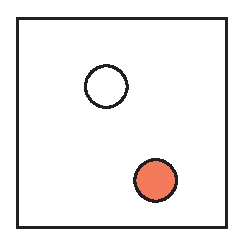
\includegraphics[width=1.5in]{sample}
  \caption{\label{fig:sample} Beispielillustration.}
\end{figure}

\begin{equation}
  \sum_{j=1}^{z} j = \frac{z(z+1)}{2}
\end{equation}

Lorem ipsum dolor sit amet, consetetur sadipscing elitr, sed diam
nonumy eirmod tempor invidunt ut labore et dolore magna aliquyam erat,
sed diam voluptua. At vero eos et accusam et justo duo dolores et ea
rebum. Stet clita kasd gubergren, no sea takimata sanctus est Lorem
ipsum dolor sit amet. Lorem ipsum dolor sit amet, consetetur
sadipscing elitr, sed diam nonumy eirmod tempor invidunt ut labore et
dolore magna aliquyam erat, sed diam voluptua. At vero eos et accusam
et justo duo dolores et ea rebum. Stet clita kasd gubergren, no sea
takimata sanctus est Lorem ipsum dolor sit amet. Lorem ipsum dolor sit
amet, consetetur sadipscing elitr, sed diam nonumy eirmod tempor
invidunt ut labore et dolore magna aliquyam erat, sed diam
voluptua. At vero eos et accusam et justo duo dolores et ea
rebum. Stet clita kasd gubergren, no sea takimata sanctus est Lorem
ipsum dolor sit amet.

Lorem ipsum dolor sit amet, consetetur sadipscing elitr, sed diam
nonumy eirmod tempor invidunt ut labore et dolore magna aliquyam erat,
sed diam voluptua. At vero eos et accusam et justo duo dolores et ea
rebum. Stet clita kasd gubergren, no sea takimata sanctus est Lorem
ipsum dolor sit amet. Lorem ipsum dolor sit amet, consetetur
sadipscing elitr, sed diam nonumy eirmod tempor invidunt ut labore et
dolore magna aliquyam erat, sed diam voluptua. At vero eos et accusam
et justo duo dolores et ea rebum. Stet clita kasd gubergren, no sea
takimata sanctus est Lorem ipsum dolor sit amet. Lorem ipsum dolor sit
amet, consetetur sadipscing elitr, sed diam nonumy eirmod tempor
invidunt ut labore et dolore magna aliquyam erat, sed diam
voluptua. At vero eos et accusam et justo duo dolores et ea
rebum. Stet clita kasd gubergren, no sea takimata sanctus est Lorem
ipsum dolor sit amet.

\begin{table}
  %% Table captions on top in journal version
  \caption{\label{tab:vis_accept} Vis Paper Acceptance Rate}
  \scriptsize
  \begin{center}
    \begin{tabular}{cccc}
      Year & Submitted & Accepted & Accepted (\%)\\
      \hline
      1994 &  91 & 41 & 45.1\\
      1995 & 102 & 41 & 40.2\\
      1996 & 101 & 43 & 42.6\\
      1997 & 117 & 44 & 37.6\\
      1998 & 118 & 50 & 42.4\\
      1999 & 129 & 47 & 36.4\\
      2000 & 151 & 52 & 34.4\\
      2001 & 152 & 51 & 33.6\\
      2002 & 172 & 58 & 33.7\\
      2003 & 192 & 63 & 32.8\\
      2004 & 167 & 46 & 27.6\\
      2005 & 268 & 88 & 32.8\\
      2006 & 228 & 63 & 27.6
    \end{tabular}
  \end{center}
\end{table}


Lorem ipsum dolor sit amet, consetetur sadipscing elitr, sed diam
nonumy eirmod tempor invidunt ut labore et dolore magna aliquyam erat,
sed diam voluptua. At vero eos et accusam et justo duo dolores et ea
rebum. Stet clita kasd gubergren, no sea takimata sanctus est Lorem
ipsum dolor sit amet. Lorem ipsum dolor sit amet, consetetur
sadipscing elitr, sed diam nonumy eirmod tempor invidunt ut labore et
dolore magna aliquyam erat, sed diam voluptua. At vero eos et accusam
et justo duo dolores et ea rebum. Stet clita kasd gubergren, no sea
takimata sanctus est Lorem ipsum dolor sit amet.


Lorem ipsum dolor sit amet, consetetur sadipscing elitr, sed diam
nonumy eirmod tempor invidunt ut labore et dolore magna aliquyam erat,
sed diam voluptua. At vero eos et accusam et justo duo dolores et ea
rebum. Stet clita kasd gubergren, no sea takimata sanctus est Lorem
ipsum dolor sit amet. Lorem ipsum dolor sit amet, consetetur
sadipscing elitr, sed diam nonumy eirmod tempor invidunt ut labore et
dolore magna aliquyam erat, sed diam voluptua. At vero eos et accusam
et justo duo dolores et ea rebum. Stet clita kasd gubergren, no sea
takimata sanctus est Lorem ipsum dolor sit amet. Lorem ipsum dolor sit
amet, consetetur sadipscing elitr, sed diam nonumy eirmod tempor
invidunt ut labore et dolore magna aliquyam erat, sed diam
voluptua. At vero eos et accusam et justo duo dolores et ea
rebum. Stet clita kasd gubergren, no sea takimata sanctus est Lorem
ipsum dolor sit amet.


\subsection{Mezcal Head}

Duis autem~\cite{Lorensen:1987:MCA} vel eum iriure dolor in hendrerit
in vulputate velit esse molestie consequat, vel illum dolore eu
feugiat nulla facilisis at vero eros et accumsan et iusto odio
dignissim qui blandit praesent luptatum zzril delenit augue duis
dolore te feugait nulla facilisi. Lorem ipsum dolor sit amet,
consectetuer adipiscing elit, sed diam nonummy nibh euismod tincidunt
ut laoreet dolore magna aliquam erat volutpat%
\footnote{Fu"snoten erscheinen an der Unterkante der Spalte. Sie
  sollten jedoch vermieden werden, da der Lesefluss gest"ort wird.}.


\subsubsection{Ejector Seat Reservation}

Ut wisi enim ad minim veniam, quis nostrud exerci tation ullamcorper
suscipit lobortis nisl ut aliquip ex ea commodo
consequat~\cite{Nielson:1991:TAD}. Duis autem vel eum iriure dolor in
hendrerit in vulputate velit esse molestie consequat, vel illum dolore
eu feugiat nulla facilisis at vero eros et accumsan et iusto odio
dignissim qui blandit praesent luptatum zzril delenit augue duis
dolore te feugait nulla facilisi.

\paragraph{Rejected Ejector Seat Reservation}

Ut wisi enim ad minim veniam, quis nostrud exerci tation ullamcorper
suscipit lobortis nisl ut aliquip ex ea commodo consequat. Duis autem
vel eum iriure dolor in hendrerit in vulputate velit esse molestie

\section{Conclusion}

Lorem ipsum dolor sit amet, consetetur sadipscing elitr, sed diam
nonumy eirmod tempor invidunt ut labore et dolore magna aliquyam erat,
sed diam voluptua. At vero eos et accusam et justo duo dolores et ea
rebum. Stet clita kasd gubergren, no sea takimata sanctus est Lorem
ipsum dolor sit amet. Lorem ipsum dolor sit amet, consetetur
sadipscing elitr, sed diam nonumy eirmod tempor invidunt ut labore et
dolore magna aliquyam erat, sed diam voluptua. At vero eos et accusam
et justo duo dolores et ea rebum. Stet clita kasd gubergren, no sea
takimata sanctus est Lorem ipsum dolor sit amet. Lorem ipsum dolor sit
amet, consetetur sadipscing elitr, sed diam nonumy eirmod tempor
invidunt ut labore et dolore magna aliquyam erat, sed diam
voluptua. At vero eos et accusam et justo duo dolores et ea
rebum. Stet clita kasd gubergren, no sea takimata sanctus est Lorem
ipsum dolor sit amet.

Lorem ipsum dolor sit amet, consetetur sadipscing elitr, sed diam
nonumy eirmod tempor invidunt ut labore et dolore magna aliquyam erat,
sed diam voluptua. At vero eos et accusam et justo duo dolores et ea
rebum. Stet clita kasd gubergren, no sea takimata sanctus est Lorem
ipsum dolor sit amet. Lorem ipsum dolor sit amet, consetetur
sadipscing elitr, sed diam nonumy eirmod tempor invidunt ut labore et
dolore magna aliquyam erat, sed diam voluptua. At vero eos et accusam
et justo duo dolores et ea rebum.


\bibliographystyle{abbrv}
%% use following if all content of bibtex file should be shown
% \nocite{*}
\bibliography{literatur}
\end{document}
\grid
